\documentclass[a4paper,12pt]{book}
\usepackage[utf8]{inputenc}
\title{}
\author{Rachel Morris}
\date{\today}

\usepackage{rachwidgets}
\usepackage{fancyhdr}
\usepackage{lastpage}
\usepackage{dirtree}
\usepackage{boxedminipage}

\setcounter{chapter}{6}
\setcounter{section}{2}
\newcommand{\laChapter}{6.3 Probability\ }

\newcommand{\laClass}{CS 211\ }
\newcommand{\laSemester}{Fall 2017\ }
\newcounter{question}

\pagestyle{fancy}
\fancyhf{}
\lhead{CS 211 Exercise}
\chead{Fall 2017}
\rhead{Ch \laChapter}
\rfoot{\thepage\ of \pageref{LastPage}}
\lfoot{\scriptsize Compiled by Rachel Morris, last updated \today}

\renewcommand{\headrulewidth}{2pt}
\renewcommand{\footrulewidth}{1pt}

\begin{document}

    %\toggletrue{answerkey}
    \togglefalse{answerkey}

    \notonkey{
    %- Team Info ------------------------------------------------------%

    \paragraph{Team name:}

    ~\\~\\
    Please write down all people in your team. ~\\

    % table %
    \begin{tabular}{ p{6cm} p{6cm} }
        1. & 2. \\ \\
        3. & 4.
    \end{tabular}
    % table %
    ~\\

    \hrulefill
    \subsection*{Grading}

    \begin{center}
        \begin{tabular}{ | l | l | l | }
            \hline
            \textbf{ Question } & \textbf{ Score } & \textbf{ Max } 
            \\ \hline
            1 &  & 3     \\ \hline
            2 &  & 3     \\ \hline
            3 &  & 3     \\ \hline
            & &  \\ \hline
            Total & & 9
            \\ \hline
        \end{tabular}
    \end{center}
    }{}

\notonkey{ \newpage }{ \hrulefill }

    %------------------------------------------------------------------%
    \section{Probability in games of chance}

    \notonkey{
        \begin{intro}{Theorem 1}
            Given a simple experiment, called a \textbf{Bernoulli trial},
            and an event that occurs with a probability $p$, if the trial is repeated
            independently $n$ times, then the probability of having exactly
            $k$ successes is
            $$ C(n, k) \cdot p^{k} \cdot (1 - p)^{n-k} $$
            \footnote{From Discrete Math by Ensley and Crawley, page 460}

            \paragraph{Example 1}
            What is the probability that in 10 successive rolls of a fair, six-sided
            die, we get exactly five results of 6?

            ~\\
            Here, we have $n = 10$, $k = 5$, and $p = \frac{1}{6}$, so:

            $$C(10, 5) \cdot (\frac{1}{6})^{5} \cdot (1 - \frac{1}{6})^{10-5}$$

            $$\frac{10!}{5!(10-5)!} \cdot (\frac{1}{6})^{5} \cdot (\frac{5}{6})^{5} $$

            $$\frac{3628800}{14400} \cdot \frac{1}{7776} \cdot \frac{3125}{7776} $$

            \begin{center}
                $ \approx 0.013 $
            \end{center}

        \end{intro}
        }{}
        
        \notonkey{ \newpage }{ \hrulefill }
        
        % -------------------------------------------------------------%
        % - QUESTION --------------------------------------------------%
        % -------------------------------------------------------------%
        \stepcounter{question}
        \begin{question}{\thequestion}{3}
            % Exercise 1

            What is the probability of getting exactly 3 heads
            on 10 tosses of a fair coin?

        \notonkey{
            \begin{center}
                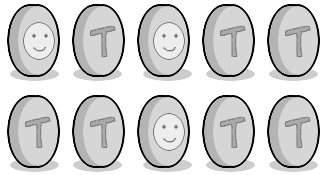
\includegraphics[width=10cm]{images/6-3-coins.png}
            \end{center}
        }{}

            ~\\~\\ \tab
            $n$, the amount of trial repeats: \solution{ 10 }{ \fitb }
            ~\\~\\ \tab
            $k$, the amount of successes (heads): \solution{ 3 }{ \fitb }
            ~\\~\\ \tab
            $p$, the probability of success: \solution{ $(1/2)$ }{ \fitb }

            ~\\~\\
            Use the formula of $ C(n, k) \cdot p^{k} \cdot (1 - p)^{n-k} $
            to find the probability.

            \solution{
                $ C(10, 3) \cdot (1/2)^{3} \cdot (1/2)^{7} = \frac{15}{128}$
            }{}
        \end{question}

        \notonkey{ \newpage }{ \hrulefill }
        
        % -------------------------------------------------------------%
        % - QUESTION --------------------------------------------------%
        % -------------------------------------------------------------%
        \stepcounter{question}
        \begin{question}{\thequestion}{3}
            % Exercise 2
            What is the probability that in seven rolls of a six-sided die,
            the result of 1 appears \textit{at least} five times?

        \notonkey{
            \begin{center}
                
\includegraphics[width=12cm]{images/6-3-dice.png}
            \end{center}
        }{}

        \notonkey{
            \begin{hint}{Hint}
                For this one, we will need to use the \textbf{rule of sums}
                to combine several outcomes: Getting 5 1's, 6 1's, OR 7 1's.
            \end{hint}
        }{}
        
            \begin{tabular}{ | c | p{4cm} | c | c | c | }
                \hline
                & & repeats $n$ & successes $k$ & probability $p$
                \\ \hline
                A &
                Getting five 1's
                    & \solution{ $ 7 $ }{ 7 }
                    & \solution{ $ 5 $ }{ 5 }
                    & \solution{ 1/6 }{ 1/6 }
                \\
                B &
                Getting six 1's
                    & \solution{ $ 7 $ }{ 7 }
                    & \solution{ $ 6 $ }{}
                    & \solution{ 1/6 }{}
                \\
                C &
                Getting seven 1's
                    & \solution{ $ 7 $ }{ 7 }
                    & \solution{ $ 7 $ }{}
                    & \solution{ 1/6 }{}
                \\ \hline
            \end{tabular}

            ~\\~\\
            Now, using the formula $ C(n, k) \cdot p^{k} \cdot (1 - p)^{n-k} $
            three different times for case (A), (B), and (C).

            ~\\~\\
            (A) \tab $ C(n, k) \cdot p^{k} \cdot (1 - p)^{n-k} $ =
            \solution{
                $C(7,5) \cdot (1/6)^{5} \cdot (5/6)^{2}$
            }{}
            
            ~\\~\\
            (B) \tab $ C(n, k) \cdot p^{k} \cdot (1 - p)^{n-k} $ =
            \solution{
                $C(7,6) \cdot (1/6)^{6} \cdot (5/6)^{1}$
            }{}
            
            ~\\~\\
            (C) \tab $ C(n, k) \cdot p^{k} \cdot (1 - p)^{n-k} $ =
            \solution{
                $C(7,7) \cdot (1/6)^{7} \cdot (5/6)^{0}$
            }{}

            ~\\~\\
            To find the probability of getting at least five 1's in seven rolls,
            add (A), (B), and (C) together. (Just write out the formula; don't solve.)

            ~\\
            $Prob($ at least five 1's $) = $
            \solution{
                $C(7,5) \cdot (1/6)^{5} \cdot (5/6)^{2} +
                C(7,6) \cdot (1/6)^{6} \cdot (5/6)^{1} +
                C(7,7) \cdot (1/6)^{7} \cdot (5/6)^{0}$
            }{ ~\\~\\ }
        \end{question}

        \notonkey{ \newpage }{ \hrulefill }
        
        % -------------------------------------------------------------%
        % - QUESTION --------------------------------------------------%
        % -------------------------------------------------------------%
        \stepcounter{question}
        \begin{question}{\thequestion}{3}
            
            % Exercise 5
            What is the probability of getting exactly one 6 on 10 tosses
            of a fair six-sided die?

            \solution{
                $n = 10$, $k = 1$, $p = (1/6)$

                $C(10,1) \cdot (1/6)^{1} \cdot (5/6)^{9} \approx 0.323 $
            }{ }
            
        \end{question}



\end{document}
